\apendice{Documentación de usuario}

\section{Introducción}

Dentro de este anexo se podrán ver los requisitos HardWare y SoftWare que tiene la aplicación para poder ser funcional, así como un manual de usuario para que cualquiera que decida usar esta aplicación tenga una guía sencilla que pueda utilizar.

\section{Requisitos de usuarios}

\subsection{Requisitos HardWare}

Para poder realizar una ejecución correcta de la aplicación se necesitará utilizar un emulador de Android que esté instalado en un ordenador con un rendimiento bastante alto, ya que este tipo de programas para emular un sistema Android al completo, exigen muchos recursos de CPU y RAM.

Otra exigencia básica para poder hacer funcionar el emulador de Android Studio es que la CPU cuente con estos requisitos mínimos:

\begin{itemize}
\item SDK Tools 26.1.1 o versiones posteriores.
\item Procesador de 64 bits.
\item CPU con compatibilidad para UG (invitado no restringido)
\item HAXM 6.2.1 o posterior (se recomienda HAXM 7.2.0 o posterior)
\item También se ha observado que en cuanto al tipo de procesador, en el caso de intel no causa ningún problema, pero con AMD, parece que sólo lo soportan los procesadores más nuevos. Esto fue probado en un procesador AMD Ryzen 2700x y no fue capaz de ejecutar el programa de emulador, en cambio en un procesador intel i7 de 8th generación funciona a la perfección.
\end{itemize}

Por supuesto, también cabe destacar que otra forma de hacer que la aplicación funcione, tratándose de Android, es usar un dispositivo que tenga una version instalada de Android 6.0 o superior. De esta manera podremos observar cómo es la experiencia al completo de ésta aplicación en un dispositivo real. 

La aplicación ha sido instalada en un dispositivo móvil Google Pixel 2 a través del emulador y en un BQ Aquaris E5 de manera física. Ambos funcionaron a la perfección bajo los requisitos mencionados anteriormente.  

\subsection{Requisitos SoftWare}

Estos son los requisitos software:

\begin{itemize}
\item Compilador de Java. Servirá para poder programar la aplicación de Android y también para ejecutar la maquina virtual Java.
\item Android Studio, ya que esta nueva herramienta proporcionada por Google permite desarrollar la aplicación en un entorno totalmente compatible. También ofrece numerosos tooltips a la hora de programar.
\item Android Developer Tools. Ésta herramienta viene incorporada en Android Studio y supone la base para poder desarrollar todo el código de Android.
\item Oracle GlassFish Server 3.0, que contendrá el servidor encargado de las respuestas al cliente.
\item Oracle VM VirtualBox, el cual servirá si no queremos instalar los programas mencionados, ya que con tenerlo todo listo en una maquina virtual podríamos ejecutar el cliente o servidor desde allí. Es importante mencionar que será necesario un ordenador con bastante potencia para poder aprovechar esta opción.
\end{itemize}

\section{Instalación}

En esta sección se encuentra detallada la guía de instalación de la aplicación.

Cabe destacar que es necesario instalar tanto el cliente en un dispositivo Android (o emulador) como el servidor en GlassFish.

\subsection{Instalación de la aplicación servidor}

Debido a que la versión de GlassFish utilizada es la misma que en anteriores versiones del proyecto, se seguirán los mismo pasos para la instalación del servidor. Dichos pasos son los siguientes:

Para instalar la aplicación en el servidor, hay que abrir la consola de administración de GlassFish tecleando en un navegador web la dirección del servidor con el puerto 4848 (http://localhost:4848 en este caso) e ir a la opción Applications.

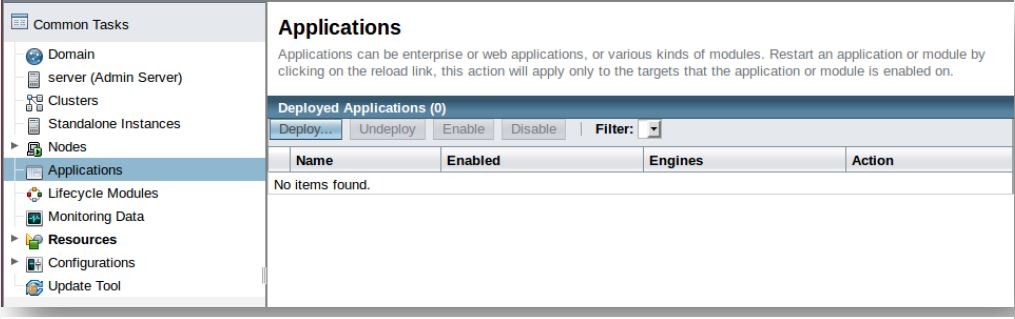
\includegraphics[width=\textwidth]{instalacionServer1.jpg}

A continuación hay que hacer click sobre el botón Deploy e indicar la ruta en la que se encuentra el archivo "osm server.war". Después, hacemos click sobre el botón OK y ya tendremos la aplicación publicada y funcionando.

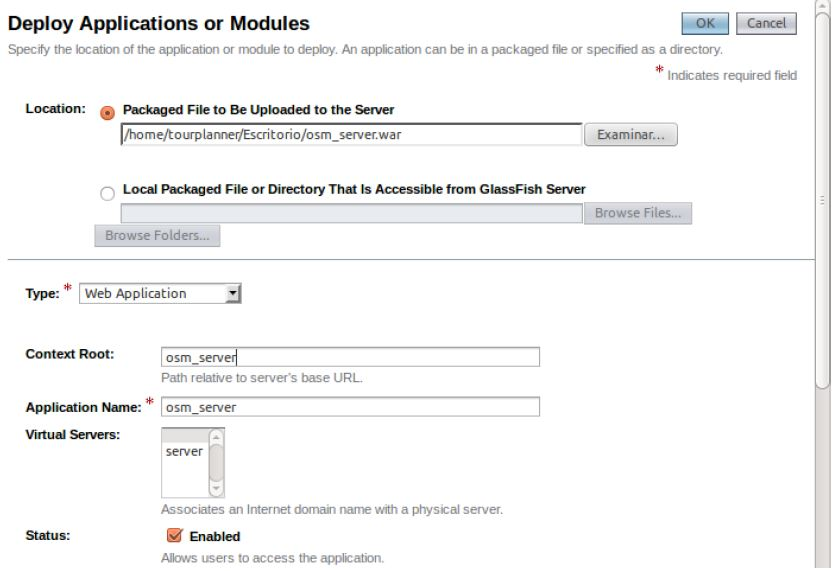
\includegraphics[width=\textwidth]{instalacionServer2.jpg}

\subsection{Instalación de la aplicación cliente}

Para realizar la instalación de nuestra aplicación Android en un dispositivo físico o un emulador, es necesario seguir estos pasos:

\begin{itemize}
\item Se necesitará, en caso de un dispositivo físico, tenerlo conectado al ordenador en el que estamos desarrollando la aplicación.
\item Una vez esté lista la aplicación, bastará con pulsar el botón de "play" en Android Studio.

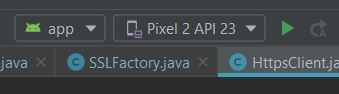
\includegraphics[width=\textwidth]{playAndroid.jpg}

\item Android Studio será el encargado de instalar el archivo.apk dentro del dispositivo y lo ejecutará directamente.
\end{itemize}

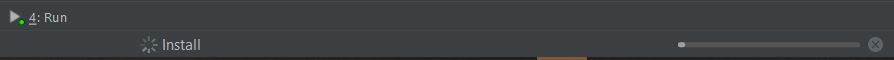
\includegraphics[width=\textwidth]{installAndroid.jpg}

Hay que tener en cuenta que para el correcto funcionamiento de la aplicación hay que seguir correctamente los pasos de compilación explicados en el apartado "Compilación del cliente", prestando especial atención al punto en el que se establece la dirección IP y puerto del servidor.

\subsection{Ejecución de la aplicación}

Para lograr que la aplicación servidor se ejecute sin la necesidad de contar con un servidor y un cliente independientes se han incluido en el USB del proyecto las maquinas virtuales correspondientes al cliente y servidor. De esta forma podremos ejecutar la aplicación con un solo ordenador.

Una de las máquinas virtuales es windows 10 y para poder ejecutar el emulador de Android, será necesario que el ordenador en el que se esté compilando posea bastante potencia, además de cumplir los requisitos mencionados en la instalación de Android Studio.

Cabe destacar que para lograr que ambas máquinas virtuales se comuniquen entre sí correctamente, se ha utilizado el programa Logmein Hamachi que nos permite crear redes virtuales entre ambas máquinas a través de Internet.

\subsubsection{Ejecución de la aplicación servidor}

Para ejecutar la aplicación servidor, hay que importar la máquina virtual Servidor - Ubuntu 18.04 LTS en un software de virtualización como VirtualBox y ejecutarla.

Una vez iniciada, introducimos la contraseña tourplanner y ejecutamos el script startGlassfish que se muestra en la ilustración, con lo que a aplicación estará ejecutándose y escuchando a la espera de peticiones.



\subsubsection{Ejecución de la aplicación cliente}

Para ejecutar la aplicación cliente, al igual que la aplicación servidor, hay que importar la máquina virtual Cliente - Windows 10 en un software de virtualización como VirtualBox y ejecutarla.

Una vez iniciada, hacer doble click sobre el acceso directo del entorno de desarrollo Android Studio. A continuación, hacemos click sobre el icono "play". Después de esto se abrirá el emulador de Android con la aplicación instalada.

\section{Manual del usuario}

En este apartado se explicará las funcionalidades que posee la aplicación, para que en un momento dado resulte más cómodo para el usuario a la hora de ser utilizada. Es importante mencionar que algunos aspectos más relacionados con pantallas en las que se establezca conexión con el servidor no se mostrarán aquí, ya que son explicaciones que ya se han desarrollado de una forma bastante completa en anteriores trabajos \cite{tfm1} y en este caso el foco se pondrá sobre los cambios de interfaz y la funcionalidad más general.

Cuando el usuario inicie la aplicación, obtendrá la siguiente pantalla:

\imagen{fotoMapa}{Imagen inicial de la aplicación al iniciarse}

Si el GPS está activado, se utilizará este servicio para determinar el foco de la aplicación. Para poder hacer esto, la aplicación solicitará permiso al dispositivo.

Si no se dispone de GPS, hay una ubicación escrita por defecto.

Tras haber accedido a esta primera pantalla, si el usuario pulsa en el botón que está arriba a la izquierda o simplemente desliza el dedo de izquierda a derecha, podrá ver el menú de opciones con el que cuenta la aplicación:

\imagen{fotoMenu}{Imagen del menú de la aplicación}

Si el usuario pulsa en la opción de Explorar el mapa:

\imagen{fotoExplorar}{Imagen de la ventana Explorar el mapa}

Aquí podrá seleccionar entre las opciones que se ofrecen, y después al pulsar en \textit{Explorar}, accederá al mapa de nuevo con las modificaciones que se han hecho tras poner estas opciones.

También se puede ver la ventana de Planificar ruta:

\imagen{fotoPlanifica}{Imagen de la ventana de Planificar ruta}

Aquí, parecido a la anterior, se podrá configurar lo que se necesite y planificar la ruta.

Si el usuario necesita cambiar alguna configuración, tendrá que acceder a la ventana de Opciones:

\imagen{fotoOpciones}{Imagen de la ventana Opciones}

Una vez aquí dentro, se pueden configurar las formas de calcular las rutas, así como las distintas preferencias que se tienen sobre ciertos puntos de interés. Pudiendo hacer que no se tengan en cuenta los que se desmarquen.

Distintas opciones sobre la forma de calcular:

\imagen{fotoOpcionesAlgo}{Imagen de la selección de Aloritmos para calcular rutas}

También la interfaz al modificar ciertas clasificaciones de puntos de interés:

\imagen{fotoOpciones2}{Imagen de las opciones de marcado sobre los puntos de interés}

El usuario también puede acceder a la parte de \textit{Mis rutas}, donde podrá almacenar rutas que le hayan gustado y cargar algunas que ya tenga almacenadas. Para poder hacer esto será necesario estar identificado.

\imagen{fotoMisrutas}{Imagen de la ventana de Mis rutas}

Por último, se puede ver las opciones que ofrece la aplicación si se decide pulsar sobre \textit{Compartir}:

\imagen{fotoRedes}{Imagen de la selección de redes sociales al compartir}